

% Section: EVALUATION
% NOTE: Evaluation section contains all subsections = setup, results, evaluation

\section{Evaluation}
\label{sec:evaluation}

In the past work~\cite{Buyksahin2013}, we studied incentive mechanisms for resource regulation within a single SN zone which corresponds to local community cloud scenario.
Here we extend our simulator to study resource regulation across multiple SN zones covering both local and federated community cloud scenarios.
In addition to simulations, we also implemented and deployed a prototype of the regulation component of Cloud Coordinator on nodes of a real community network using the Community-Lab testbed~\cite{Neumann2012} provided by the CONFINE project~\cite{Braem2013}.
However, as only a handful of nodes are made available currently, the analysis of our proposed system on greater scale using the real prototype system is too limited.
Therefore, we focus here on reporting results from the simulation experiments, where our scenario could be extended to a community cloud consisting of 1,000 nodes.

%%%%%%%%%%%%%%%%%%%%%%%%%%%%%%%%%%%%%%%
\subsection{Experiment Setup}
We simulate a community network comprising of 1,000 nodes which is divided into 100 zones and each zone has one super node and nine ordinary nodes.
The zones are distributed in a small world topology where each zone is neighbour to 10 other zones.
This approximation holds well for real world community networks as, for example, topology analysis of Guifi.net~\cite{Vega2012} shows that the ratio of super node to ordinary nodes is approximately 1 to 10. 
Each ordinary node in the simulation can host a number of VM instances that allows users' applications to run in isolation.
Nodes in the zone have two main attributes, one is capacity which is the number of available VM instances, and other is sharing behaviour which is how many instances are shared with other nodes.
Table~\ref{tab:ONconf} shows the different configurations for each of the nine ONs in each zone.
Nodes with low, medium and high capacity host 3, 6 and 9  VM instances respectively and they exhibit selfish, normal or altruistic behaviour sharing one-third, two-thirds or all of their VM instances.
For example, node ON2 has medium capacity with 6 instances and exhibits selfish behaviour reserving 4 instances for itself and contributing only 2 to the system.     

\begin{table}[htb]
\renewcommand{\arraystretch}{1.3}
\footnotesize
\centering
     \caption{Configuration for each node in a zone with shared and total instances}
    \begin{tabular}{@{} cc c c c c @{}}
    \hline
    {Node Behaviour} & {Shared} & Small capacity & Medium capacity & Large capacity   \\  \hline
    {Selfish} & 33\% 	& ON1 (1/3) & ON2 (2/6) & ON3 (3/9) & \\ 
	{Normal} & 66\% 	& ON4 (2/3) & ON5 (4/6) & ON6 (6/9) & \\ 
	{Altruistic} & 100\%& ON7 (3/3) & ON8 (6/6) & ON9 (9/9) & \\ \hline
    \label{tab:ONconf}
    \end{tabular}
\end{table}

When the experiment runs, nodes make requests for resources proportional to their capacity asking for two-thirds of their capacity.
For instance nodes with capacity of 3, 6 and 9 VM instances request 2, 4 and 6 instances respectively.
Nodes request instances for fixed duration and after transaction is complete wait briefly before making further requests.

\subsection{Experimental Results}

We evaluate the impact of the effort-based incentive mechanisms in the system in simulation experiments and discuss the results below.
We study the success ratio, i.e. number of requests fulfilled versus total requests, and the overall resource utilisation in the system.

%%%%%%%%%%%%%%%%%%%%%%%%%%%%%%%%%%%%%%%
\subsubsection{Ratio of Successful Requests}

Table~\ref{tab:ONresult} shows the success ratio for requests made by different nodes analysed both with the effort-based and contribution-based incentive mechanisms. 
We first notice that the success ratio values decrease as the capacity of the nodes increases. 
This is explained by the fact that nodes with greater capacity request more instances and so have a higher chance getting rejected either because there are not many resources available in the system or because the requesting nodes do not have sufficient credit.

Moreover, when we compare success ratio for nodes having as capacity increases, we observe greater variation in the case of contribution-based incentives.
For instance, for the normal sharing behaviour the values range from 66\% to 97\% for contribution-based incentives, but from 86\% to 90\% for effort-based incentives.
This is explained by the fact that contribution-based approach does not take heterogeneity of nodes into account and penalises nodes with low capacity as they cannot contribute as much to the system as others.
These results indicate that effort-based incentives ensure \emph{fairness} in the system since the nodes with the same sharing behaviour are treated equally irrespective of their capacity.

\begin{table}[tb]
\renewcommand{\arraystretch}{1.3}
\footnotesize
\centering
  \caption{Success ration of nodes for different configurations with effort and contribution based incentives}
    \begin{tabular}{@{} cc c c c c @{}}
    \cline{1-5}
     {Node Behaviour} & {Incentives} & Small capacity & Medium capacity & Large capacity   \\ \hline 
     {\multirow{2}{*}{Selfish}} &
	 {effort-based} & 54\% & 53\% & 50\% & \\ 
	 {} &
	 {contribution-based} & 66\% & 59\% & 39\% & \\ \hline
 	 {\multirow{2}{*}{Normal}} &
	 {effort-based} & 90\% & 91\% & 86\% & \\ 
	 {} &
	 {contribution-based} & 97\% & 77\% & 66\% & \\ \hline
 	 {\multirow{2}{*}{Altruistic}} &
	 {effort-based} & 97\% & 94\% & 86\% & \\ 
	 {} &
	 {contribution-based} & 97\% & 85\% & 65\% & \\ \hline
    \label{tab:ONresult}
    \end{tabular}
\end{table}


%%%%%%%%%%%%%%%%%%%%%%%%%%%%%%%%%%%%%%%
\subsubsection{Breakdown of Request Responses}
% Graph 
\begin{figure}[bth]
   \centering
   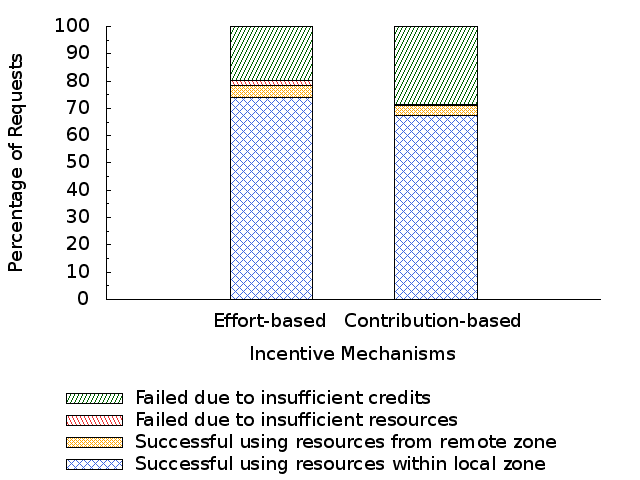
\includegraphics[width=3.0in,keepaspectratio]{graph_requestRatio}
   \caption{Breakdown of outcome of requests with effort and contribution based mechanisms}
   \label{fig:req_breakdown}
\end{figure}

Figure~\ref{fig:req_breakdown} shows the breakdown of successful and rejected requests. 
The success ratio is higher for effort-based incentives.
Moreover, contribution-based mechanism has greater share of requests rejected because of lack of credit.
This indicates that effort-based incentives result in better efficiency as more resources remain utilised.
Another observation is that majority of requests are fulfilled using resources from local zone with very few requests forwarded to other zones. 

 

%%%%%%%%%%%%%%%%%%%%%%%%%%%%%%%%%%%%%%%
\subsubsection{Resource Utilisation}
%% Graph 
\begin{figure}[htb]
   \centering
   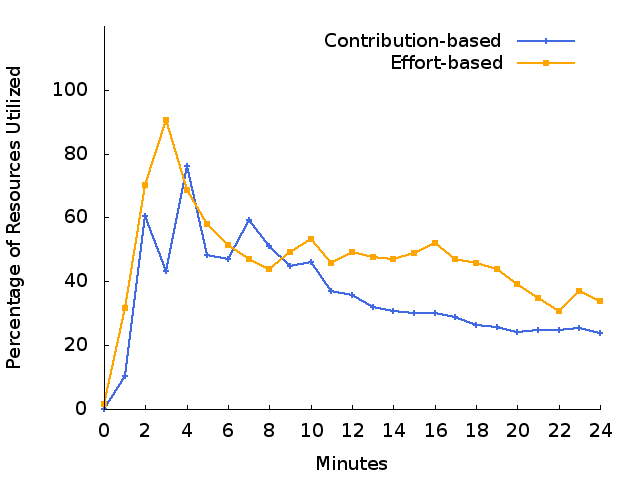
\includegraphics[width=3.0in,keepaspectratio]{graph_resourceUtil}
   \caption{Resource utilisation along 24 minutes of the experiment}
   \label{fig:res_util}
\end{figure}

Figure~\ref{fig:res_util} shows the proportion of resources utilised in the system along the execution of a 24 minutes experiment for effort and contribution based approach. In the start all nodes have enough credit and the resource utilisation is high. Then it drops to below 60\% at around the 12\textsuperscript{th} minute. 
Then, since most of the nodes completed their transactions and consumed their credits, the utilisation decreases significantly. The effort-based approach though achieve a higher resource utilisation during that time. 


%%%%%%%%%%%%%%%%%%%%%%%%%%%%%%%%%%%%%%%
\subsubsection{Nodes Selection Policies}
%% Graph 
\begin{figure}[htb]
   \centering
   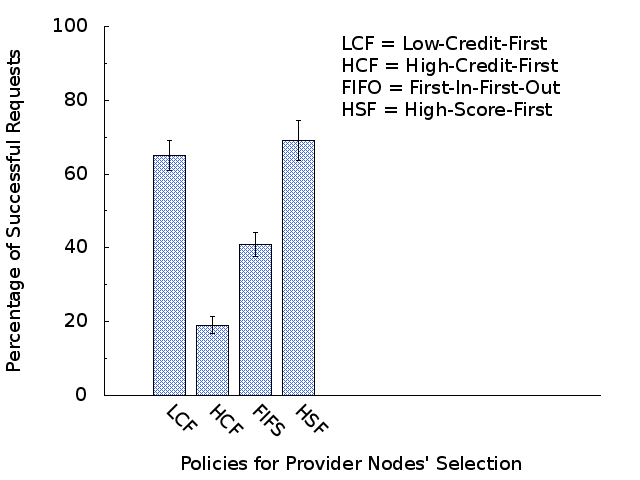
\includegraphics[width=3.0in,keepaspectratio]{graph_selectionMec}
   \caption{Success ratio comparison of provider ON selection strategies}
   \label{fig:selection_mech}
\end{figure}

Figure~\ref{fig:selection_mech} shows the effect of different node selection policies on the success ratio when using effort-based incentives. 
High-credit-first and first-in-first-out policies perform poorly since they do not consider the credits of the nodes and so fail in ensuring a balanced distribution across the system. 
The low-credit-first and high-credit-first policies performs better since they give preference to nodes with low credit allowing them to earn more so that they can be successful with their future requests.

